% ----------------------------------------------------------
% Introdução (exemplo de capítulo sem numeração, mas presente no Sumário)
% ----------------------------------------------------------
\chapter[Introdução]{Introdução}
%\addcontentsline{toc}{chapter}{Introdução}
% ----------------------------------------------------------
\par Este capítulo apresenta a motivação deste trabalho, os objetivos definidos e a metodologia adotada.

\section{Motivação}

\par Gamificação é a utilização de conceitos de jogos em aplicações com outros contextos, estes conceitos são: ganho de pontos, \textit{ranking}, troféus e conquistas, assim como processos que devem ser concluídos, e, quando são finalizados com sucesso, algum tipo de recompensa é recebida, aumentando a motivação e o interesse dos usuários \cite{robson2015all}. Dito isto, \textit{softwares} utilizam esta ideia para estimular usuários a realizar determinado processo e/ou continuar utilizando seus serviços, aplicando lógicas que dão recompensas quando forem finalizadas, desta forma incentivam seus usuários a continuar utilizando a solução criada \cite{hamari2014does}. Devido ao crescimento do interesse por este termo (Figura \ref{fig:gamification-google-trends}) nos últimos anos \cite{groh2012gamification}, aplicações com contextos não relacionados a jogos vem adotando a ideia dos \textit{games}, alguns exemplos são: Duolingo, aplicativo para aprender idiomas e Foursquare, aplicativo para verificar classificações de locais. Estas aplicações possuem fins totalmente diferentes, porém, aplicam lógicas semelhantes de gamificação, que é a continuidade da utilização para se obter mais conquistas. As conquistas são chamadas de ofensivas no Duolingo e de pontos no Foursquare.

\begin{figure}[H]
    \centering
    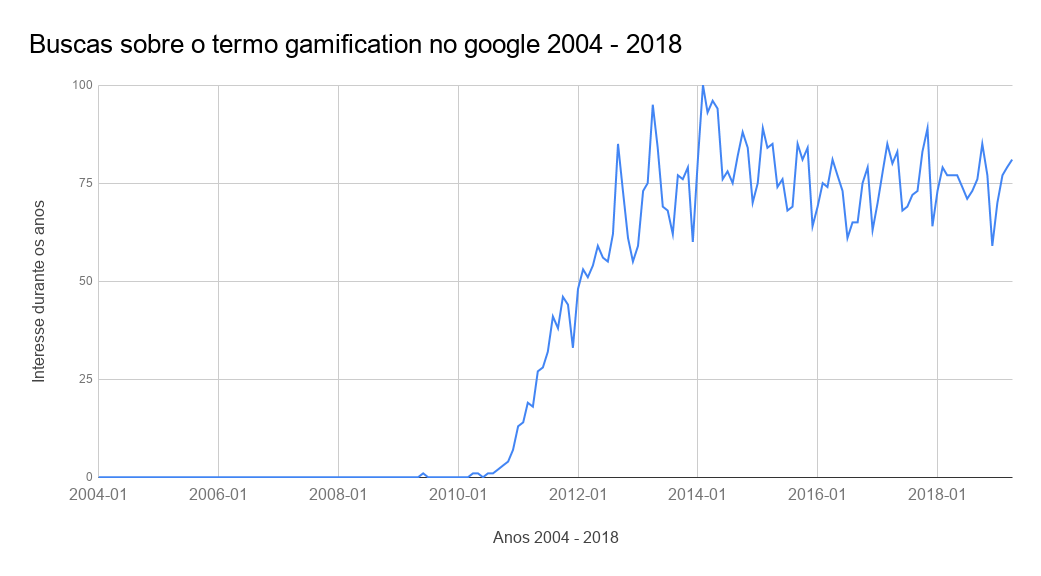
\includegraphics[scale=0.4]{src/imagens/cap1/gamification-google-trends.png}
    \caption{Consultas sobre a palavra \textit{gamification} durante os anos}
    \label{fig:gamification-google-trends}
    \fonte{Origem de dados: Google Trends \citeonline{google-trends}}
\end{figure}

\par A lógica gamificação do aplicativo Duolingo se baseia em metas, estas metas são atingidas após a execução de uma sequência de sentenças, podendo variar entre o idioma definido como nativo e o estudado. A meta diária, é definida na primeira execução do aplicativo, todavia pode ser alterada a qualquer momento. A meta limita a quantidade de execuções diárias para ser atingida, ou seja, para se atingir a meta diária é necessário realizar no mínimo X execuções completas. Quando a meta é atingida, a contagem de ofensivas é aumentada em um, isto mantém usuários determinados a não perder sua ofensiva, devido a falta de utilização, e por outro lado o usuário desenvolve outro idioma. Existe também um ranking de usuários, o que estimula a competição, e assim aumenta a utilização do aplicativo \cite{melo2016eficiencia}.

\par O aplicativo Foursquare tem como objetivo exibir locais e suas classificações, estas classificações são feitas pelos próprios usuários, quando estes realizam \textit{check-in}. Ao realizar este processo, que é inserir sua localização no aplicativo, pontos são obtidos, e é disponibilizada a opção de avaliação do local, para que no futuro, quando este for o resultado de pesquisas, as avaliações feitas previamente sejam exibidas, para que o usuário possa escolher qual o melhor local, que atenda as suas necessidades naquele momento. A lógica de gamificação aplicada neste aplicativo, é, quanto maior a frequência de \textit{check-ins} realizados mais pontos são obtidos. Um ranking também está presente nesta aplicação, estimulando assim a competição e a continuidade da utilização para que mais lugares sejam avaliados\cite{huotari2012defining}.

\par Baseado nisto, a gamificação é útil diversas aplicações, porém, é necessário um contexto para que estes padrões como: pontos, rankings, troféus e conquistas, sejam aplicados para cativar e/ou estimular os usuários, o que pode não ser um processo simples dependendo do objetivo da aplicação. O \textit{framework} Esfinge Gamification disponibiliza uma solução para o problema citado, abstraindo a complexidade da criação destas funcionalidades. Este tem como objetivo desacoplar qualquer lógica de gamificação da aplicação que utilizar suas funcionalidades, permitindo que o programador não se preocupe em como criá-las no código que está desenvolvendo, apenas insira anotações do \textit{framework} onde precisar de comportamentos de gamificação \citeonline{esfingegamification2011} e estes serão desencadeados conforme Figura \ref{fig:esfingesample}, onde o método \textit{answerQuestion()} possui a anotação \textit{PointsToUser}, esta anotação dá 10 pontos do tipo \textit{ANSWER} ao usuário atual configurado no \textit{framework}, porém, toda a lógica para a adição destes pontos é realizada pelo Esfinge Gamification, isto é transparente a aplicação.

\begin{figure}[H]
    \centering
    \begin{java}

// Interface com anotacao do framework
public interface Questionnaire {
    @PointsToUser(name = "ANSWER", quantity = 10)
    public void answerQuestion(String answer);
}

public class QuestionnaireImpl implements Questionnaire {
    // Implementacao omitida
}

public static void main(String[] args) {
    // Configuracao do framework omitida
    Questionnaire q = (Questionnaire) GameProxy.createProxy(new QuestionnaireImpl());
    q.answerQuestion("Gamification works!");
}
\end{java}
    \caption{Exemplo Esfinge Gamification}
    \label{fig:esfingesample}
    \fonte{Adaptado de \citeonline{esfingegamification2011}}
\end{figure}

\par Adicionar restrições de uso aumenta o empenho dos usuários a fim de conseguir novas funcionalidades ou recursos que ficam disponíveis conforme a utilização, isto é reconhecido na área da Psicologia Comportamental como reforço negativo  \cite{skinner1990behavior}. Geralmente, jogos que possuem restrições têm os recursos desbloqueados conforme o progresso do personagem ou a consecução de algum objetivo, aplicações que implementam lógicas de gamificação costumam possuir esta abordagem para atingir os objetivos citados anteriormente a partir de regras de autorização. Atualmente o Esfinge Gamification não possui funcionalidades deste tipo, portanto, este trabalho é motivado pela oportunidade da criação de funcionalidades de autorização baseadas em conquistas existentes no \textit{framework}, para que, caso mecanismos de autorização sejam necessários em aplicações que utilizem a solução, estes poderão ser adicionados por meio de anotações, e assim, desencadear comportamentos de autorização transparentes a aplicação, seguindo a filosofia do Esfinge Gamification.

\section{Problema}

\par O problema identificado foi a falta de opções para adicionar autorização em aplicações que utilizam lógica de gamificação. Uma oportunidade de melhoria foi a integração entre os \textit{frameworks} Esfinge Gamification e Esfinge Guardian.

% Section Objetivo Geral!
\section{Objetivo Geral}
\par O objetivo deste trabalho é prover mecanismos de autorização baseados em conquistas para o Esfinge Gamification, ou seja, é a criação de funcionalidades de autorização a partir dos dados de gamificação disponibilizados pelo \textit{framework}.
% precisa disso será? para que o desenvolvedor não tenha que preocupar-se com a criação destes mecanismos e utilize uma interface simples disponibilizada pelo \textit{framework} para aplicar estas funcionalidades em projetos. 

% Section Objetivo Especifico!
\section{Objetivo Espec\'ifico}

\par Para a realização deste objetivo foram estabelecidas metas específicas:
\begin{itemize}
    \item Integração entre os \textit{frameworks} Esfinge Gamification e Esfinge Guardian, a partir da criação de componentes de autorização para o Esfinge Gamification;
    \item Criação de anotações para obter controle de acesso baseado em conquistas utilizando os recursos disponibilizados pelo \textit{framework} Esfinge Gamification.
\end{itemize}

\section{Metodologia}

\par O desenvolvimento dos componentes adicionais para o \textit{framework} tem como etapa inicial a integração entre o Esfinge Guardian e o Esfinge Gamification, após isto, a criação de anotações para aumentar a abstração das funcionalidades de autorização oferecidas pela solução, realizando assim uma interface amigável, e permitindo ao desenvolvedor aplicar regras de autorização de uma maneira simples e eficaz. Para realizar estes objetivos, técnicas de reflexão e anotação em java foram utilizadas.

\section{Organização do trabalho}

Este Trabalho está organizado nos seguintes capítulos:

\begin{itemize}
	\item Capítulo 2: Contém a fundamentação teórica necessária para entender os assuntos abordados no capítulo de desenvolvimento;
	\item Capítulo 3: Possui o desenvolvimento do trabalho, como o objetivo foi concretizado;
	\item Capítulo 4: Neste capítulo o desenvolvimento é testado e sua teoria valiada com um caso de uso;
	\item Capítulo 5: Aborda as conclusões e considerações finais a respeito deste trabalho.
\end{itemize}